\documentclass[tikz,border=2pt]{standalone}
\usepackage{amsmath,amssymb}
\usepackage{tikz}
\usetikzlibrary{arrows.meta}

\begin{document}
% The optimal solution is the feasible point with the best objective value: sliding the
% objective line as far as possible, it last touches the region at the corner (20, 60).
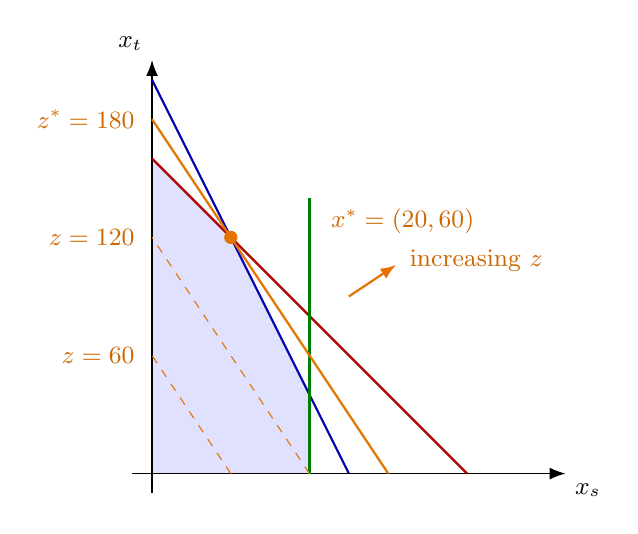
\begin{tikzpicture}[x=0.05cm, y=0.05cm, every node/.style={font=\small}, >={Latex[length=2mm]}]
	\fill[blue!12] (0,0) -- (40,0) -- (40,20) -- (20,60) -- (0,80) -- cycle;
	\draw[->] (-5,0) -- (105,0) node[below right] {$x_s$};
	\draw[->] (0,-5) -- (0,105) node[above left] {$x_t$};
	\draw[blue!70!black, thick] (50,0) -- (0,100);
	\draw[red!70!black, thick] (80,0) -- (0,80);
	\draw[green!50!black, thick] (40,0) -- (40,70);
	\draw[orange!90!black, dashed] (20,0) -- (0,30);
	\draw[orange!90!black, dashed] (40,0) -- (0,60);
	\draw[orange!90!black, thick] (60,0) -- (0,90);
	\node[orange!80!black, font=\small, anchor=east] at (-2,30) {$z=60$};
	\node[orange!80!black, font=\small, anchor=east] at (-2,60) {$z=120$};
	\node[orange!80!black, font=\small, anchor=east] at (-2,90) {$z^\ast=180$};
	\draw[->, orange!90!black, thick] (50,45) -- (62,53);
	\node[orange!80!black, font=\small, anchor=west] at (63,54) {increasing $z$};
	\fill[orange!90!black] (20,60) circle (2.4pt);
	\node[orange!80!black, font=\small, anchor=west] at (43,64) {$x^\ast=(20,60)$};
	\end{tikzpicture}
\end{document}
